%********************************************************************************
%       Preamble Information
%********************************************************************************
\documentclass[11pt, twocolumn]{article}
\usepackage[T1]{fontenc}
\usepackage[utf8]{inputenc}
\usepackage{mathpazo}
\usepackage{multicol}
\setlength\columnsep{20pt}

\usepackage{hyperref}
\hypersetup{
    colorlinks=true,
    linkcolor=blue,
    filecolor=magenta,      
    urlcolor=blue,
    citecolor=black
    }
% Used to include graphic images into LaTeX
\usepackage{graphicx}
% Tells the compiler to search in the images/ 
% folder for any included figures
\graphicspath{ {./images/} }

% Make lists more compact
% (from pandoc template)
\providecommand{\tightlist}{\setlength{\itemsep}{0pt}\setlength{\parskip}{0pt}}

% Prevent overfull lines
\setlength{\emergencystretch}{1em}

% No indentation and space between paragraph
\setlength{\parindent}{0.0in}
%\setlength{\parskip}{0.04in}
% Have space between paragraph
\setlength{\parskip}{11pt}

% Margin support
\usepackage[margin=0.75in]{geometry}

% header and footer
\usepackage{fancyhdr}

\newcommand{\thelabnumber}{HW3}
\newcommand{\thetitle}{HW3: Computer History}
% Update this line with your name 
\newcommand{\theauthor}{Aidan Butcher \\ Dylan DeVault}

% Write title and author
\title{{\large } \thetitle}
\author{\theauthor}
\date{\today}

\pagestyle{fancy}
\fancyhf{}
\fancyfoot[R]{\thepage}
\fancyfoot[C]{HW3}
\fancyfoot[L]{CSE/IT 101 HW3}
\renewcommand{\footrulewidth}{1pt}
\renewcommand{\headrulewidth}{0pt}
\fancypagestyle{firstpage}{%
  \fancyhf{}% clear default for header and footer
  \fancyfoot[R]{\thepage}
  \fancyfoot[C]{HW3}
  \fancyfoot[L]{CSE/IT 101}
  \renewcommand{\footrulewidth}{1pt}
    \renewcommand{\headrulewidth}{0pt}
}

%********************************************************************************
%      Begin Document
%********************************************************************************
\begin{document}
\maketitle

\thispagestyle{firstpage}

%********************************************************************************
%      Report Content
%********************************************************************************
\section{Introduction}
The topic chosen for this paper is Artificial Intelligence and Robotics. Artificial
Intelligence, or AI for short, are machines that demonstrate intelligence. They are
capable of understanding their environments and can take actions in response to
their environments. They are made by computer scientists to solve problems typical
programs cannot solve. They can also be created to learn, allowing them to adapt to
new situations.

\section{Time Period}
Artificial Intelligence were first theorized by Warren McCullouch and Walter Pitts
in 1943 with their formal design for Turing complete artificial neurons. Research
of AI was started in 1956 at Dartmouth College after the invention of digital
computers. The reason AI were researched is because of the possibility of creating
an electronic brain. It was also theorized that the creation of general artificial
intelligence would be capable of doing any work a person could do. The intent was to
replace all, if not most jobs, with AI, but the difficult of the task ended up being
far greater than anticipated. So research slowed until 1980, when expert system, a
form of AI program that managed to simulate the analytical skill and knowledge of
humans. This was followed by another lapse in research until the late 20th century
and early 21st century when AI began to solve specific problems. As faster computers,
the internet, better algorithms, and more data was found, AI research gained a lot
of popularity. AI have become so prevalent that they are now used in video games,
solving analytical problems, board games, search engines, advertisement, and much
more.

\section{Computer Hardware}

The hardware used for AI is typically computers capable of using specific programming
languages. Since digital computers were first made accessible, researchers were
attempting to create AI. Now they can be run on nearly any computer, depending on the
task(s) they are created for. Very complicated tasks tend to require more powerful
machines like supercomputers or quantum computers. Simple tasks may only require
basic computers with a processor and enough memory to run the AI.

\begin{figure}
    \centering
    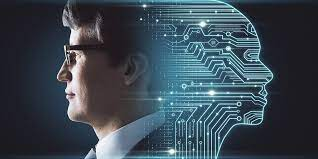
\includegraphics[width=0.45\textwidth]{AI}
    \caption{Picture of AI Visualized}
    \label{fig:AI}
\end{figure}

\subsection{Computer Software}
Describe the type of software used for your chosen topic, if any, and state any uses
of the software that your topic had. If your topic does not have or use software, 
describe why it doesn't use software and how it functions without it.

\subsection{Conclusion}
Conclude your research paper with any reflections on what you learned about your 
topic. Was this what you expected to find? Did you find any facts that surprised you?
You may add other personal reflections about the topic here.

%********************************************************************************
%      Report Content
%********************************************************************************
\bibliographystyle{acm}
\bibliography{sources}


\end{document}